\documentclass[a4paper, 12pt]{book}
\usepackage{graphicx}
\usepackage[french]{babel}
\usepackage[utf8]{inputenc}
\usepackage[T1]{fontenc}
\usepackage{multirow}
\usepackage{listings}
\usepackage{float}
\usepackage{url}
\usepackage[french]{algorithm}
\usepackage{style/myalgorithm}
\usepackage{amsmath,amsfonts,amssymb}
\newcommand{\fBm}{\emph{fBm}~}
\newcommand{\etal}{\emph{et al.}~}
\newcommand{\glAd}{\emph{GL4D}~}
\newcommand{\apiopengl}{API OpenGL\textsuperscript{\textregistered}~}
\newcommand{\opengl}{OpenGL\textsuperscript{\textregistered}~}
\newcommand{\opengles}{OpenGL\textsuperscript{\textregistered}ES~}
\newcommand{\clang}{langage \texttt{C}}
\newcommand{\codesource}{\textsc{Code source}~}
\floatstyle{ruled}
\newfloat{programslist}{htbp}{locs}
\newcommand{\listofprograms}{\listof{programslist}{Liste des codes source}}
\newcounter{program}[subsection]
\renewcommand{\theprogram}{\arabic{chapter}.\arabic{program}}

\newenvironment{program}[1]{
  \if\relax\detokenize{#1}\relax
  \gdef\mycaption{\relax}
  \else
  \gdef\mycaption{#1}
  \fi
  \refstepcounter{program}
  \addcontentsline{locs}{section}{#1}
  \footnotesize
}{
  \begin{description}
    \item[\codesource \theprogram]--~\mycaption
  \end{description}
}

\begin{document}
\begin{titlepage}
  \begin{center}
    \begin{tabular*}{\textwidth}{l@{\extracolsep{\fill}}r}
      
\includegraphics[height=1.5cm]{images/m2ise.png}
    \end{tabular*}
    \small 
    \rule{\textwidth}{.5pt}~\\
    \large 
    \textsc{Université Paris 8 - Vincennes à Saint-Denis}\vspace{0.5cm}\\
    \textbf{Master Informatique des Systèmes Embarqués}\vspace{3.0cm}\\
    \Large
    \textbf{Memoire de projet tuteuré}\vspace{1.5cm}\\
    \large
    \textbf{Fakhri \textsc{YAHIAOUI} - Roman \textsc{BOURSIER}}\vspace{1.5cm}\\
    Date de soutenance : le 09/06/2020\vspace{1.75cm}\\
  \end{center}\vspace{1.5cm}~\\
  \begin{tabular}{ll}
    \hspace{-0.45cm}Tuteur -- Université~:~&~Farès \textsc{BELHADJ}\\
  \end{tabular}
\end{titlepage}
\frontmatter
\chapter*{Résumé}
\markboth{\sc Résumé}{}
\addcontentsline{toc}{chapter}{Résumé} 

A faire en dernier ...


\chapter*{Remerciements}
\markboth{\sc Remerciements}{}
\addcontentsline{toc}{chapter}{Remerciements} 

Idem ...

%% Table des matières
\tableofcontents

\mainmatter
\chapter*{Introduction}
\markboth{\sc Introduction}{}
\addcontentsline{toc}{chapter}{Introduction}

\section{Contexte}
Dans le cadre de notre projet de fin d'étude, nous souhaitons utiliser des modèles d’apprentissage automatique (ex. Deep Learning) afin de produire un moteur de rendu capable d’adopter une stylisation « type » telle que la peinture chinoise. Dans un premier temps, il s’agira de proposer un modèle d’abstraction des peintures sélectionnées comme base d’apprentissage et d’utiliser le couple « peinture originale » / « abstraction » pour l’entraînement. Par la suite, un moteur de rendu d’abstractions sera connecté au réseau profond qui produira une peinture sur la base de l’abstraction.

Le modèle généré devra d'une part adopter la stylisation retenue mais aussi interpréter l'abstraction d'origine.

\section{Résultats et solutions apportées}


%% Technologies
\section{Technologies existante}
Todo -- Chapeau


%% ETAT DE L'ART
\section{Etat de l'art}
Todo -- Chapeau

\subsection{Google DeepDream}
https://fr.wikipedia.org/wiki/DeepDream
https://github.com/google/deepdream

\subsection{Google quickdraw}
https://quickdraw.withgoogle.com/

\subsection{Semantic Image Synthesis with SPADE (GauGAN)}
https://arxiv.org/pdf/1903.07291.pdf

\subsection{Coco dataset}
Versions of COCO-Stuff

\subsection{Le transfert de style neuronal}

Cette technique fut décrite par Leon A. Gatys dans son article "A Neural Algorithm of Artistic Style".~\cite{DBLP:journals/corr/GatysEB15a}

Celle-ci utilise trois images, la première est l'image d'entrée (bruit), la seconde représente le style de référence (comme une peinture par exemple), la dernière correspond à l'image que l'on souhaite transformer.

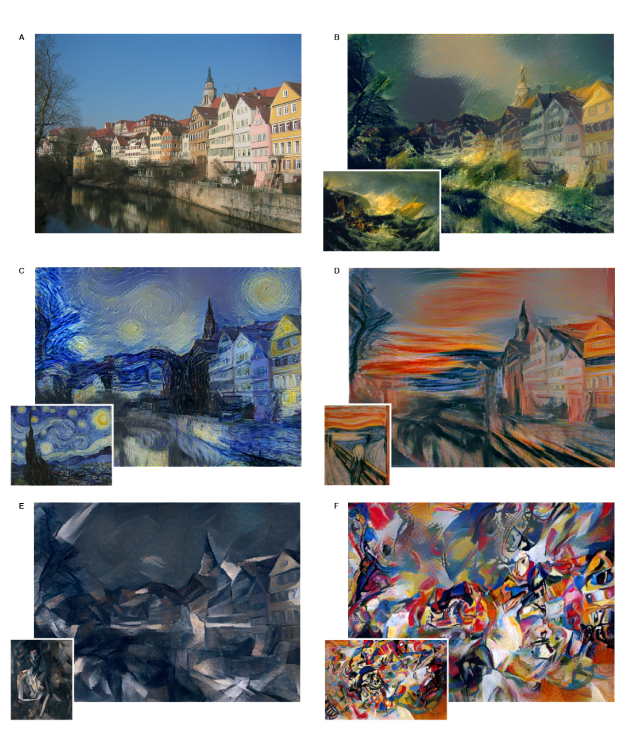
\includegraphics[width=0.7\linewidth]{images/neuronal-algorithm-artistic-style.png}

Le principe consiste à définir deux fonctions de distance. La première décrit comment le contenu de deux images sont différentes, et la seconde réprésente la différence de style. On obtient alors deux images, une pour le style souhaité, une pour le contenu.

L'objectif est de transformer l'image d'entrée en minimisant la distance avec l'image de contenu et avec l'image de style. On obtiens alors par rétropogation, une image qui correspond au contenu de l'image d'origine et au style souhaitée.

Cela nécessite la création d'un réseau convolutionnel, en effet le modèle doit être en mesure de capturer les invariances et de définir les caractéristiques de l'images (chats vs chien) afin d'en obtenir une compréhension générale.

\subsection{Le transfert de style neuronal}
https://www.groundai.com/project/stable-and-controllable-neural-texture-synthesis-and-style-transfer-using-histogram-losses/2
https://www.groundai.com/project/automated-deep-photo-style-transfer/1

\subsection{Texture transfert}

\subsection{Segmentation non-supervise}
\subsection{Semantique segmentation}
http://datahacker.rs/top-10-github-papers-semantic-segmentation/
https://www.arxiv-vanity.com/papers/1603.01768/

 
 
\subsection{Engouement des gans}
https://github.com/hindupuravinash/the-gan-zoo

\subsection{image translation}

\subsection{Image analogies}
A. Hertzmann, C. E. Jacobs, N. Oliver, B. Curless, and D. H.
Salesin. Image analogies. 2001.
https://medium.com/syncedreview/visual-attribute-transfer-through-deep-image-analogy-6f0ffa5e9e09

\subsection{Scene Completion}
http://graphics.cs.cmu.edu/projects/scene-completion/

\subsection{Image segmentation et conditionnal gan}
https://www.arxiv-vanity.com/papers/1612.00215/



\chapter{Conclusion et Perspectives\label{chap-conclusion}}

\bibliographystyle{alpha}
\bibliography{memoire}
\end{document}
